\documentclass[conference]{IEEEtran}
\IEEEoverridecommandlockouts
\usepackage{graphicx}
\usepackage{amsmath,amssymb}
\usepackage{booktabs}
\usepackage{cite}
\usepackage{url}
\usepackage[hidelinks]{hyperref}
% generated by paper/make_tables.py -- do not edit
\newcommand{\aciCapMaxPct}{8.2}
\newcommand{\aciCapMeanPct}{0.9}
\newcommand{\batBestModel}{Moirai-2.0}
\newcommand{\batFmHi}{82.7}
\newcommand{\batFmLo}{81.9}
\newcommand{\batLgbm}{80.4}
\newcommand{\batNaive}{76.7}
\newcommand{\batVariantSpread}{1.8}
\newcommand{\bestRegretErcoLoad}{1.99}
\newcommand{\calNativeHi}{1.48}
\newcommand{\calNativeLo}{0.19}
\newcommand{\calNativeN}{8}
\newcommand{\calNativeSig}{8}
\newcommand{\chronosBeatsLgbmSeries}{4}
\newcommand{\commonDays}{274}
\newcommand{\confEightyCovHi}{0.807}
\newcommand{\confEightyCovLo}{0.801}
\newcommand{\confEightyISHi}{0.404}
\newcommand{\confEightyISLo}{0.397}
\newcommand{\confEightyWorstHourHi}{9.3}
\newcommand{\confEightyWorstHourLo}{8.6}
\newcommand{\confNinetyCovHi}{0.906}
\newcommand{\confNinetyCovLo}{0.900}
\newcommand{\confNinetyRangeHi}{0.93}
\newcommand{\confNinetyRangeLo}{0.87}
\newcommand{\costBest}{4.03}
\newcommand{\costBestModel}{Chronos-2}
\newcommand{\ctxCommonDaysErco}{212}
\newcommand{\ctxCostNinety}{4.13}
\newcommand{\ctxCostSeven}{4.48}
\newcommand{\ctxCostTwentyEight}{4.13}
\newcommand{\ctxNmaeNinety}{0.076}
\newcommand{\ctxNmaeSeven}{0.081}
\newcommand{\ctxNmaeTwentyEight}{0.077}
\newcommand{\ctxWidthGainPct}{7}
\newcommand{\detReductionHi}{38}
\newcommand{\detReductionLo}{27}
\newcommand{\eightyWidthIncreasePct}{6}
\newcommand{\ercotDropped}{30}
\newcommand{\imputedCovDiffPp}{0.3}
\newcommand{\nRivals}{7}
\newcommand{\nRivalsSig}{6}
\newcommand{\nTopDisagree}{4}
\newcommand{\nTopDisagreeSig}{1}
\newcommand{\nativeCovMaxAll}{0.81}
\newcommand{\nativeCovMinAll}{0.73}
\newcommand{\nativeEightyCov}{0.784}
\newcommand{\nativeEightyIS}{0.408}
\newcommand{\nativeEightyKupPass}{15}
\newcommand{\nativeEightyUnder}{71}
\newcommand{\nativeEightyWorstHour}{14.7}
\newcommand{\nativeEightyWorstHourMax}{43}
\newcommand{\nmaeBestFmCisoSolar}{0.070}
\newcommand{\nmaeBestFmErcoLoad}{0.035}
\newcommand{\nmaeChronosErcoWind}{0.121}
\newcommand{\nmaeLgbmCisoSolar}{0.067}
\newcommand{\nmaeLgbmErcoWind}{0.172}
\newcommand{\nmaeNaiveErcoWind}{0.204}
\newcommand{\nmaeOperatorErcoLoad}{0.024}
\newcommand{\opNativeRegret}{23.2}
\newcommand{\opRegretErco}{1.11}
\newcommand{\rhoHi}{1.00}
\newcommand{\rhoLo}{0.45}
\newcommand{\rhoPinHi}{1.00}
\newcommand{\rhoPinLo}{0.69}
\newcommand{\rivalSecond}{TiRex}
\newcommand{\rivalSecondDiff}{0.12}
\newcommand{\rivalSecondHi}{0.26}
\newcommand{\rivalSecondLo}{-0.01}
\newcommand{\rivalThird}{Moirai-2.0}
\newcommand{\rivalThirdDiff}{0.18}
\newcommand{\rivalThirdHi}{0.28}
\newcommand{\rivalThirdLo}{0.08}
\newcommand{\seedSdMax}{0.28}
\newcommand{\shortfallHi}{12.0}
\newcommand{\shortfallLo}{3.3}
\newcommand{\shortfallMean}{5.1}
\newcommand{\testDays}{304}
\newcommand{\topThreePairsTotal}{18}
\newcommand{\topThreeSigPairs}{2}
\newcommand{\windGainPct}{24}
\newcommand{\worstHourWNinety}{5.9}
\newcommand{\worstHourWOneEighty}{7.4}
\newcommand{\worstHourWThirty}{4.2}


\begin{document}

\title{Are Time-Series Foundation Models Operationally Reliable? Conformal Calibration and Decision Value for History-Only Day-Ahead Load, Solar and Wind Forecasting}

\author{\IEEEauthorblockN{Tanishq Singh Sisodiya}
\IEEEauthorblockA{\textit{Affiliation (TODO)}\\
City, Country \\
email (TODO)}}

\maketitle

\begin{abstract}
Grid operators size reserves and commit storage from forecast quantiles, yet time-series foundation models (TSFMs) are judged mainly on point accuracy. We ask whether their uncertainty can be used as delivered. Four TSFMs (Chronos-2, TimesFM-2.5, Moirai-2.0, TiRex) and four trained baselines forecast day-ahead load, solar and wind for ERCOT and CAISO from EIA-930 history only, on a ten-month test period that begins after every checkpoint was published. Every model's quantiles pass through four conformal calibration methods and then through a newsvendor reserve rule and a battery-firming program. Three findings emerge. First, without weather inputs the leading TSFMs are the most accurate history-only models for load and wind. Second, native quantiles are rarely calibrated: at their own 80\% level only \nativeEightyKupPass\% of model--series cases pass a coverage test, and the worst hour of the day misses by \nativeEightyWorstHour\ points on average. Third, a per-hour conformal layer fixes average coverage at little extra width and lowers reserve cost for all \calNativeN\ models; the cost ranking follows the quantile loss at the operating level more closely than point accuracy.
\end{abstract}

\begin{IEEEkeywords}
Foundation models, probabilistic forecasting, conformal prediction, operating reserves, energy storage.
\end{IEEEkeywords}

\section{Introduction}
Zero-shot time-series foundation models now match or beat task-specific models on many energy benchmarks \cite{prior_ercot_tsfm,prior_fets,prior_consumer}. Those benchmarks report median errors and at most a proper score such as CRPS, but operators use the tails: reserve requirements, battery commitments and risk limits are set from quantiles. An accurate but overconfident model under-procures reserve; an underconfident one wastes capacity. Prior work applied split conformal prediction to one TSFM on one dataset \cite{prior_conformal_ercot} and fine-tuned one TSFM for one feeder decision \cite{prior_dfl}; the calibration and operating value of the current model generation across targets and conformal methods has not been measured.

We ask: \textbf{RQ1} how accurate are current zero-shot TSFMs against trained models on history-only day-ahead load, solar and wind? \textbf{RQ2} are their native intervals calibrated, and which conformal method restores nominal coverage with the narrowest intervals as conditions change between winter and summer? \textbf{RQ3} when intervals drive reserve sizing and battery scheduling, which model and calibration pair is cheapest, and does that follow the accuracy ranking? Contributions:
\begin{enumerate}
\item A leakage-controlled benchmark of four TSFMs, four baselines and the balancing authority's load forecast on six EIA-930 series, tested after every checkpoint's publication.
\item A comparison of native and four conformal calibrations at equal nominal levels, including coverage by hour of day and miss clustering.
\item A decision-value evaluation of reserve cost and battery profit with paired block-bootstrap confidence intervals, and a decomposition that links reserve cost to the quantile loss at the operating level.
\item Code, pinned configurations and outputs that rebuild every table and figure.\footnote{\url{https://github.com/TanishqX-404/tsfm-grid-calibration}}
\end{enumerate}

\begin{figure}[t]
\centering
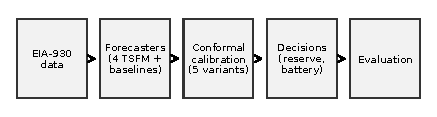
\includegraphics[width=\columnwidth]{figures/F1_pipeline.pdf}
\caption{Pipeline. Every model writes the same quantile table; calibration and decision code is shared, so cost differences come only from the forecasts.}
\label{fig:pipeline}
\end{figure}

\section{Data and Protocol}
\textbf{Data.} We use hourly EIA-930 demand and solar and wind generation \cite{eia930} for ERCOT and CAISO from the PUDL tables \cite{pudl} (six series). Timestamps are in local standard time; gaps of up to 3\,h are interpolated; solar and wind are normalized by a trailing 90-day maximum (a causal capacity proxy) and load by its training mean. Training runs from July 2019 to December 2024, validation from January to October 2025 and test from 1 November 2025 to 31 August 2026 (\testDays\ daily origins; September and October are not in the test year). Days whose context or target contains a longer gap are dropped for every model; EIA-930 lacks 5 December 2025 for ERCOT, which removes \ercotDropped\ ERCOT test days.

\textbf{Information set.} Forecasts are \emph{history-only}: no weather or other covariates. The forecast for day $D$ is issued at midnight using the 28 days before $D$ and covers the 24 hours of $D$ (lead times 1--24\,h, so horizon equals hour of day). Market day-ahead forecasts are made about 14\,h earlier, when ERCOT and CAISO day-ahead markets close on the morning of $D-1$; our early horizons are therefore close to nowcasts, which flatters every model, persistence-like ones most. Solar night hours, defined causally from data because CAISO's EIA-930 solar profile drifts by about 1.5\,h between 2022 and 2025, are excluded from accuracy, coverage and width; in the reserve problem they carry zero reserve and zero error.

\textbf{Models.} The TSFMs are Chronos-2 \cite{ansari2025chronos2}, TimesFM-2.5 \cite{das2024timesfm}, Moirai-2.0-R-small \cite{liu2025moirai2} and TiRex \cite{auer2025tirex}, run zero-shot from pinned checkpoints. Baselines, each trained on its own series only, are seasonal naive (lag 24\,h for solar and wind, 168\,h for load, with empirical residual quantiles), LightGBM quantile regression \cite{ke2017lightgbm} on 24/48/168-h lags and calendar features (Optuna, 30 trials), and N-HiTS \cite{challu2023nhits} and PatchTST \cite{nie2023patchtst} with a multi-quantile loss (three seeds each). N-HiTS memorized its single training series and its quantiles collapsed on validation, so for load and wind it uses early stopping on the last 90 training days. All models output quantiles $0.1,\dots,0.9$; the median is the point forecast. We also report the balancing authority's day-ahead load forecast.

\textbf{Leakage control.} Table~\ref{tab:ckpt} lists when each checkpoint's weights were committed; all precede the test start (Moirai-2.0's weights were published in August 2025, before its technical report). No documented pretraining corpus contains EIA-930 or CAISO data. An ERCOT load set in the Chronos corpus was a held-out benchmark for Chronos \cite{ansari2024chronos}; we cannot rule out its use by Chronos-2 and TiRex, but it predates our test period.

\begin{table}[t]
\caption{Checkpoint dates (weights file at the pinned revision).}
\label{tab:ckpt}
\centering\footnotesize
\begin{tabular}{lcc}
\toprule
Model & Weights committed & Report (arXiv) \\
\midrule
TiRex & 2025-05-26 & 2505.23719 \\
Moirai-2.0 & 2025-08-06 & 2511.11698 \\
TimesFM-2.5 & 2025-10-01 & 2310.10688 \\
Chronos-2 & 2025-10-30 & 2510.15821 \\
\bottomrule
\end{tabular}

\end{table}

\textbf{Protocol.} All settings (LightGBM hyper-parameters, calibration step sizes, the fixed-reserve share, and each model's calibration variant and battery interval level in Table~\ref{tab:dec}) were chosen on validation, frozen and tagged; the test period was evaluated once. The foundation models reproduced their test forecasts bit-for-bit in a second, independent run.

\section{Calibration and Decision Layers}
\textbf{Calibration.} Conformalized quantile regression (CQR) \cite{romano2019cqr} scores each past day by how far the outcome fell outside the model's interval, $s=\max(\hat q^{lo}-y,\ y-\hat q^{hi})$, and widens (or narrows) the interval by a quantile $Q$ of past scores: $[\hat q^{lo}-Q,\ \hat q^{hi}+Q]$. Each calibrator is fit separately per series and per hour of day and updated daily from days whose outcomes are known. The four variants differ only in how $Q$ is chosen. \emph{Split CQR} takes the empirical quantile of the last $W=90$ days. \emph{NexCP} \cite{barber2023nexcp} weights older days less ($0.99^{\text{age}}$). \emph{ACI} \cite{gibbs2021aci} nudges the target miscoverage up after each covered day and down after each miss, $\alpha_{t+1}=\alpha_t+\gamma(\alpha-\text{err}_t)$. \emph{PID} denotes the proportional, quantile-tracking term of conformal PID control \cite{angelopoulos2023pid}, which moves $Q$ itself by a fixed step after each hit or miss; we do not use its integral or forecasting terms. Energy series are not exchangeable, so split CQR and NexCP coverage is empirical; ACI and quantile tracking guarantee long-run average coverage for any sequence (quantile tracking for bounded scores). The native band $[\hat q_{0.1},\hat q_{0.9}]$ is the only native interval the models provide, so we compare native and conformal intervals at the 80\% level and report conformal intervals alone at 90\%. One-sided bounds for the decision layer apply the same method to the nearest native quantile (0.9 or 0.1), so native reserve bounds sit at 0.9 even when the decision needs 0.95.

\textbf{Tests.} The Kupiec test checks whether the share of misses equals the nominal rate \cite{kupiec1995}; the Christoffersen test checks whether a miss makes the next miss more likely \cite{christoffersen1998}. Kupiec is applied to all hourly misses of a series and assumes independence, which autocorrelated misses violate, so its rejection rates are inflated. Christoffersen is applied to each hour's daily miss sequence (median $p$ over hours).

\textbf{Reserve sizing.} With reserve cost $c_R$ and shortfall penalty $c_S$, the expected-cost-optimal upward reserve is the $\tau^*=1-c_R/c_S$ quantile of the forecast error (newsvendor). Reserve $R_h$ is the calibrated one-sided bound at $\tau^*$ minus the median (upper bound for load, lower for solar and wind), and daily cost is $J=\sum_h [c_R R_h + c_S (e_h-R_h)^+]$ with error $e_h$ in the reserve direction, in normalized units. Whenever the bound lies beyond the median,
\begin{equation}
J/c_S=\textstyle\sum_h \rho_{\tau^*}(e_h-R_h)+(1-\tau^*)\sum_h e_h,
\label{eq:decomp}
\end{equation}
where $\rho_\tau$ is the pinball loss: reserve cost is the quantile loss of the $\tau^*$ bound plus a bias term. We report $\tau^*=0.95$ ($c_S/c_R=20$) and a fixed rule $R_h=k\hat y_h$ with $k$ tuned on validation as a simple reference.

\textbf{Battery firming.} A solar or wind plant of capacity 1 with a 0.5/1.0 battery (90\% round-trip) commits a day-ahead schedule by a linear program on the calibrated lower bound under a stated two-level time-of-use price; a greedy real-time rule covers deviations, shortfalls pay three times the price and surplus sells at half. Profit is reported as a share of an oracle that plans on the true outcome.

\section{Results}
\textbf{RQ1: accuracy.} Table~\ref{tab:acc} gives test nMAE. Chronos-2, Moirai-2.0 and TiRex are the most accurate history-only models on load and wind; on ERCOT wind Chronos-2 reaches \nmaeChronosErcoWind\ against \nmaeLgbmErcoWind\ for LightGBM and \nmaeNaiveErcoWind\ for seasonal naive, and on both wind series the TSFMs are \windGainPct\% more accurate than LightGBM on average. On pinball loss Chronos-2 beats LightGBM significantly (Diebold--Mariano with Harvey correction \cite{diebold1995dm,harvey1997hln}, Holm-adjusted, 5\%) on \chronosBeatsLgbmSeries\ of six series, while only \topThreeSigPairs\ of \topThreePairsTotal\ comparisons among the three leading TSFMs are significant. On solar, lagged LightGBM is as accurate as the TSFMs (CAISO: \nmaeLgbmCisoSolar\ vs.\ \nmaeBestFmCisoSolar). ERCOT's own day-ahead load forecast, which uses weather, remains the most accurate (\nmaeOperatorErcoLoad\ vs.\ \nmaeBestFmErcoLoad); the CAISO operator row is not comparable, because EIA-930 CAISO demand has diverged from CAISO's forecast definition since 2022.

\begin{table}[t]
\caption{Test nMAE (normalized MAE of the median; solar daytime only) and mean native 80\% coverage. Bold: lowest per series; underlined: pinball loss not significantly worse than the best (DM, Holm, 5\%). The operator forecast is a point forecast with no native interval.}
\label{tab:acc}
\centering\footnotesize\setlength{\tabcolsep}{2.6pt}
\resizebox{\columnwidth}{!}{\begin{tabular}{lccccccc}
\toprule
Model & ERCOT L & ERCOT S & ERCOT W & CAISO L & CAISO S & CAISO W & Cov$_{80}$ \\
\midrule
Seasonal naive & 0.095 & 0.104 & 0.204 & 0.066 & 0.075 & 0.155 & 0.78 \\
LightGBM & 0.051 & \underline{0.097} & 0.172 & 0.034 & \underline{\textbf{0.067}} & 0.134 & 0.79 \\
N-HiTS & 0.040 & 0.126 & 0.135 & 0.042 & 0.085 & 0.114 & 0.73 \\
PatchTST & 0.038 & 0.116 & 0.130 & 0.035 & 0.095 & \underline{0.113} & 0.80 \\
Chronos-2 & \underline{0.036} & \underline{0.095} & \underline{\textbf{0.121}} & \underline{0.032} & \underline{0.070} & \underline{0.111} & 0.78 \\
Moirai-2.0 & \underline{0.036} & \underline{\textbf{0.095}} & 0.124 & \underline{\textbf{0.031}} & \underline{0.070} & \underline{0.110} & 0.79 \\
TimesFM-2.5 & 0.044 & \underline{0.103} & 0.127 & 0.037 & 0.076 & \underline{0.112} & 0.78 \\
TiRex & \underline{\textbf{0.035}} & \underline{0.100} & \underline{0.121} & 0.033 & \underline{0.074} & \underline{\textbf{0.109}} & 0.81 \\
\midrule
Operator (BA) & 0.024 & -- & -- & 0.096 & -- & -- & 0.01 \\
\bottomrule
\end{tabular}
}
\end{table}

\textbf{RQ2: calibration.} Table~\ref{tab:cal} pools eight models and six series. Averages hide the problem: the native 80\% band covers \nativeEightyCov\ on average, and PatchTST and TiRex are close to nominal. But \nativeEightyUnder\% of model--series pairs under-cover, only \nativeEightyKupPass\% pass the Kupiec test, and the worst hour of the day misses by \nativeEightyWorstHour\ points on average (up to \nativeEightyWorstHourMax). At the same 80\% level, conformal intervals cover \confEightyCovLo--\confEightyCovHi, are only \eightyWidthIncreasePct\% wider, score slightly better on the interval (Winkler) score (\confEightyISLo--\confEightyISHi\ vs.\ \nativeEightyIS), and cut the worst-hour gap to \confEightyWorstHourLo--\confEightyWorstHourHi\ points. At 90\% they cover \confNinetyCovLo--\confNinetyCovHi\ on average (\confNinetyRangeLo--\confNinetyRangeHi\ over series). Differences among the four methods are small (width within 2\%) and we did not test them formally; adaptive methods mainly reduce miss clustering. We therefore recommend the simplest, split CQR with a 30--90-day window: a shorter window gives better hour-of-day coverage (worst-hour gap \worstHourWThirty, \worstHourWNinety\ and \worstHourWOneEighty\ points for $W=30,90,180$ days at 90\%). ACI capped its interval on \aciCapMeanPct\% of test days, and removing EIA-imputed hours changes coverage by at most \imputedCovDiffPp\ points.

\begin{table}[t]
\caption{Calibration pooled over eight models and six series (test). IS: interval (Winkler) score; Worst hr: mean largest hour-of-day coverage gap from nominal; Kup./Chr.: share of model--series pairs passing the Kupiec and Christoffersen tests at 5\%.}
\label{tab:cal}
\centering\footnotesize\setlength{\tabcolsep}{2.4pt}
\begin{tabular}{lccccccc}
\toprule
Variant & Cov. & Range & Width & IS & Worst & Kup. & Chr. \\
 & & & & & hr (pp) & (\%) & (\%) \\
\midrule
\multicolumn{8}{l}{\emph{Target 80\% (native band $[\hat q_{0.1},\hat q_{0.9}]$ available)}} \\
Native & 0.784 & 0.66--0.87 & 0.276 & 0.408 & 14.7 & 15 & 71 \\
Split CQR & 0.801 & 0.75--0.83 & 0.293 & 0.404 & 8.6 & 69 & 71 \\
NexCP & 0.807 & 0.78--0.83 & 0.293 & 0.402 & 9.3 & 44 & 75 \\
ACI & 0.804 & 0.77--0.84 & 0.294 & 0.400 & 9.1 & 62 & 83 \\
PID & 0.802 & 0.78--0.83 & 0.290 & 0.397 & 8.6 & 71 & 90 \\
\midrule
\multicolumn{8}{l}{\emph{Target 90\% (no native interval)}} \\
Split CQR & 0.900 & 0.87--0.91 & 0.375 & 0.482 & 5.9 & 71 & 81 \\
NexCP & 0.906 & 0.89--0.92 & 0.378 & 0.480 & 6.1 & 56 & 85 \\
ACI & 0.905 & 0.88--0.93 & 0.379 & 0.478 & 5.9 & 65 & 90 \\
PID & 0.900 & 0.88--0.92 & 0.370 & 0.475 & 7.3 & 60 & 90 \\
\bottomrule
\end{tabular}

\end{table}

\begin{figure*}[t]
\centering
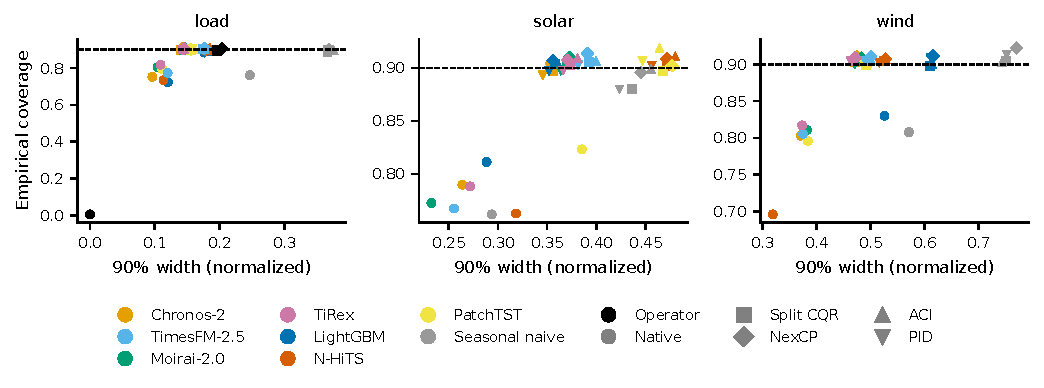
\includegraphics[width=\textwidth]{figures/F2_coverage_width.pdf}
\caption{Coverage of 90\% intervals against normalized width (test), averaged over the two regions; the native points are the 80\% band. Colour: model; marker: calibration variant; dashed: nominal.}
\label{fig:covwidth}
\end{figure*}

\textbf{RQ3: decision value.} Table~\ref{tab:dec} reports reserve cost at $\tau^*=0.95$ per series and, in the mean columns, over the \commonDays\ days on which all six series have forecasts, the same days the paired bootstrap uses. Calibration lowers reserve cost for all \calNativeSig\ models, by \calNativeLo--\calNativeHi\ normalized units per day (paired moving-block bootstrap \cite{kunsch1989}, 7-day blocks, 95\% intervals excluding zero); part of this gain comes from reaching the 0.95 level that native quantiles cannot. Against the fixed-percentage rule, calibrated intervals are \detReductionLo--\detReductionHi\% cheaper. \costBestModel\ has the lowest mean cost (\costBest); \rivalSecond\ costs \rivalSecondDiff\ more per day (95\% CI \rivalSecondLo\ to \rivalSecondHi, not significant) and \rivalThird\ \rivalThirdDiff\ more (CI \rivalThirdLo--\rivalThirdHi); \nRivalsSig\ of \nRivals\ differences are significant. Shortfall occurs in \shortfallMean\% of hours on average, close to the 5\% implied by $\tau^*$. For ERCOT load the operator's point forecast with conformal intervals is cheaper than any model (regret \opRegretErco\ vs.\ \bestRegretErcoLoad); without calibration it cannot size reserve at all (regret \opNativeRegret). In battery firming (Fig.~\ref{fig:battery}) the TSFMs recover \batFmLo--\batFmHi\% of oracle profit (best: \batBestModel), against \batLgbm\% for LightGBM and \batNaive\% for seasonal naive; the calibration variant changes profit by at most \batVariantSpread\ points, far less than the commitment level.

\begin{table*}[t]
\caption{Test reserve cost at $\tau^*=0.95$ (normalized units per day) with each model's validation-selected calibration, per series (all days of each series) and mean over the \commonDays\ common days, with native intervals and the fixed rule for comparison; Battery: profit as \% of oracle (solar and wind). Bold: lowest; underlined: not significantly different from the lowest (paired block bootstrap, 95\%).}
\label{tab:dec}
\centering\footnotesize\setlength{\tabcolsep}{4pt}
\begin{tabular}{lccccc}
\toprule
Model & Cal. & Native & Fixed & Short. & Battery \\
 & cost & cost & rule & (\%) & (\% orc.) \\
\midrule
Chronos-2 & \textbf{3.98} & 4.23 & 5.78 & 5.3 & 82.4 \\
TiRex & 4.14 & 4.32 & 5.82 & 5.1 & 82.5 \\
Moirai-2.0 & 4.15 & 4.49 & 5.70 & 5.9 & \textbf{82.7} \\
PatchTST & 4.41 & 4.85 & 6.49 & 4.7 & 81.5 \\
TimesFM-2.5 & 4.43 & 5.01 & 6.29 & 4.8 & 81.9 \\
N-HiTS & 4.66 & 6.16 & 6.41 & 4.6 & 80.1 \\
LightGBM & 4.75 & 5.37 & 7.71 & 5.5 & 80.4 \\
Seasonal naive & 6.48 & 7.69 & 9.46 & 4.8 & 76.7 \\
\bottomrule
\end{tabular}

\end{table*}

\begin{figure}[t]
\centering
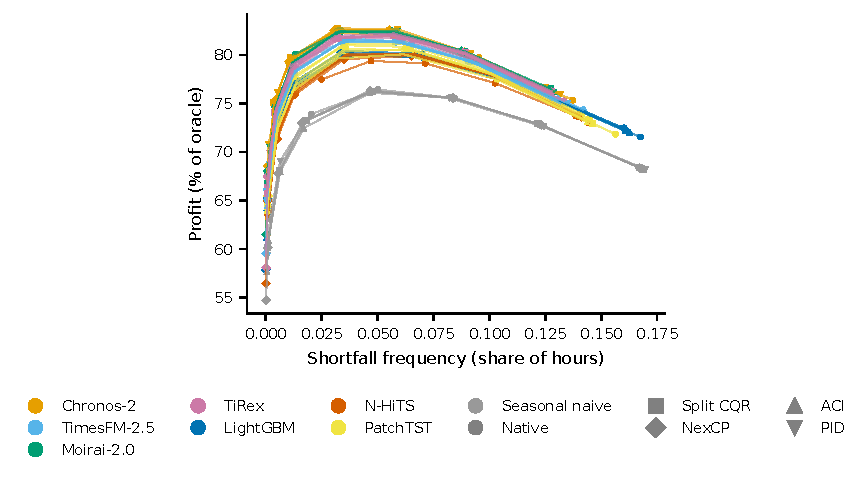
\includegraphics[width=\columnwidth]{figures/F3_battery_frontier.pdf}
\caption{Battery firming frontier (test, mean over solar and wind series): profit as \% of oracle against shortfall frequency; each line traces one model and calibration pair across interval levels 0.5--0.99.}
\label{fig:battery}
\end{figure}

\textbf{Accuracy vs.\ cost.} By (\ref{eq:decomp}), reserve cost measures the quantile loss at $\tau^*$, not the median error, so the two rankings need not agree. Across series the Spearman correlation between cost rank and nMAE rank is \rhoLo--\rhoHi, but between cost rank and the pinball loss of the $\tau^*$ bound it is \rhoPinLo--\rhoPinHi\ (Fig.~\ref{fig:rank}). The most accurate model is not the cheapest in \nTopDisagree\ of six series, but the cost gap is significant in only \nTopDisagreeSig; with eight models, rank correlations are imprecise, so we read this as ``accuracy is an unreliable proxy for operating cost'' rather than as a reversal.

\begin{figure}[t]
\centering
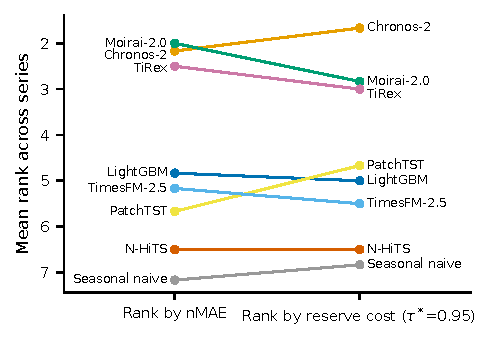
\includegraphics[width=\columnwidth]{figures/F4_rank_slope.pdf}
\caption{Mean rank across series by nMAE (left) and by reserve cost at $\tau^*=0.95$ with the validation-selected calibration (right), test period.}
\label{fig:rank}
\end{figure}

\textbf{Ablations.} Shortening the TSFM context from 28 to 7 days raises nMAE from \ctxNmaeTwentyEight\ to \ctxNmaeSeven\ and reserve cost from \ctxCostTwentyEight\ to \ctxCostSeven; 90 days gives \ctxNmaeNinety\ and \ctxWidthGainPct\% narrower calibrated intervals at unchanged cost (\ctxCostNinety; common days only). The seed spread of the trained baselines is small (regret s.d.\ $\le$\,\seedSdMax).

\section{Discussion and Limitations}
From history alone, zero-shot TSFMs are the most accurate of the models we tested for load and wind, but their quantiles should not be used as reserve requirements as delivered. A per-hour conformal layer of a few hundred lines of NumPy, running in seconds on a CPU, fixes average coverage and lowers reserve cost for every model; it matters most for the worst-calibrated models. Limitations: forecasts are history-only and issued at midnight rather than at market close, so they understate the lead time and omit the weather forecasts operators rely on (especially for solar and wind); the fixed-percentage rule is a weak reference, and empirical-residual and operator-style dynamic reserve baselines remain to be added; prices are stated, not market prices; results cover two balancing authorities and ten months; baselines are single-series models and N-HiTS uses target-specific training settings; the capacity proxy is a trailing maximum; and the CAISO demand definition in EIA-930 limits the operator comparison to ERCOT.

\section{Conclusion}
Across six ERCOT and CAISO series, current foundation models are the most accurate history-only day-ahead forecasters for load and wind, yet their quantiles are rarely calibrated as delivered. Conformal calibration is cheap, restores nominal coverage on average at equal levels with little extra width, and lowers reserve cost for every model. Chronos-2 and TiRex gave the lowest reserve cost, and the cost ranking tracked the quantile loss at the operating level more closely than point accuracy.

\section*{Acknowledgment}
AI-assisted tools (Anthropic Claude) were used for code development and for drafting parts of the text; the authors reviewed and verified all content. (TODO: confirm wording against the IEEE policy on AI-generated content.)

\bibliographystyle{IEEEtran}
\bibliography{refs}

\end{document}
